% Notes on writing:
% 
% * Use one sentence per line (no hard word wrapping), which makes merging different versions a lot easier.
% * Use \EM{}, \PO{} or \EA{} to add your personal comments or todos.
% * Using Git, the easiest way is probably to create your own branch and merge updates into the master branch. For Mac, see https://mac.github.com



% From DoW (603773_DOW_2013-08-05[3].pdf, p.17):
%
% D1.3) Report on LBKD model and method in the climate change domain: 
% A survey of the key publications, approaches, software and resources on Literature-Based Knowledge Discovery will be conducted. 
% In addition, any work in this area specifically related to climate change will be surveyed. 
% This will result in survey paper on LBKD in the field of climate change [month 6]


\documentclass[11pt,oneside,a4paper]{report}
\usepackage{natbib}
\usepackage[nottoc]{tocbibind} 
\usepackage{graphicx}
\usepackage{hyperref}
\usepackage{url}

%\usepackage{todonotes}
% To hide all notes use 
\usepackage[disable]{todonotes}


\newcommand{\EM}[1]{\todo[inline,author=EM,color=yellow]{#1}}
\newcommand{\PO}[1]{\todo[inline,author=PO,color=blue]{#1}}
\newcommand{\EA}[1]{\todo[inline,author=EA,color=green]{#1}}


\begin{document}

\title{Deliverable D1.1:\\ Literature-based Knowledge Discovery\\in Climate, Marine and Environmental Science}
\author{Erwin Marsi, Pinar \"Ozt\"urk, Elias Aamot}
\date{Version 1.0 -- \today}
\maketitle

\abstract{
This deliverable surveys the state-of-the art in literature-based knowledge discovery.
This includes a survey of key publications, approaches, software and resources related to literature-based knowledge discovery in general as well any work specifically in the area of climate, marine and environmental science. 
The purpose is to (1) prevent duplication of efforts, (2) to promote reuse of existing theory, practice and resources, (3) to identify potential bottlenecks early on and (4) to generally make sure that the results from work on WP1 will reach or exceed the state-of-the-art in the field.
Chapter 1 surveys text mining in general as a combination of information retrieval, information extraction, natural language processing and data mining.
The remainder of the chapter is focused on text mining in biomedicine, as almost all work on literature mining originates from this area.
A couple of text mining applications are described, followed by a description of the major tasks in text mining, i.e. entity detection, relation and event extraction.
The closely related fields of machine reading and open information extraction are Briefly discussed.
Chapter 2 provides an in depth survey of literature-based knowledge discovery.
Approaches are grouped into domain-independent, concept-based and relation extraction-based -- ranging from purely statistical methods to those involving sophisticated natural language processing.
The largely unresolved issue of system evaluation is reviewed.
Chapter 4 survey work on text mining in the domain of climate, marine and environmental science.
Efforts specifically in this area turn out to be few and far between, so tools, resources and applications in related areas are taken into consideration here, for example, from ecology, geology and paleobiology.
%Finally, chapter 5 discusses some ongoing and planned work in WP1 as far as related to the content of this deliverable.
}

\tableofcontents

\chapter*{Acknowledgements}

Parts of the chapter on literature-based knowledge discovery are from the draft version of the master thesis of Elias Aamot, who is advised by Pinar \"Ozt\"urk and Erwin Marsi.    


\chapter{Introduction}

Scientific publications are sources of knowledge encoded in text.
Each one contributes to our collective knowledge and they are often considered the main end product of scientific activity.
Quantity and quality of publications, for instance measured through journal impact factors, are nowadays the primary performance indicator for individual researchers, research groups, research centres or universities.  
The ``publish or perish'' culture is one of the driving forces behind the ever growing amount of scientific publications.
Other factors include the ease of electronic publication as well as the many computational tools speeding up modern science, from search engines to DNA sequencing.
As a result, the scientific literature is growing at an astounding rate of four papers per minute on average.
In many disciplines, ths means has become almost impossible for individual researchers to keep track of all new developments reported in the literature, even in their relatively narrow fields of expertise.

Search engines alone, although an essential tool for bibliographic research, are not sufficient to cope with the massive amount of scientific literature available.
Many search queries result in thousands of hits and sifting through all these documents by hand to locate the relevant pieces of information is practically infeasible.
This is where techniques and applications from the field of natural language processing (NLP) may offer a better solution.
\emph{Question-Answering}, for example, attempts to directly find the correct answer in a large text collection, in resonse to question posed by the user.
\emph{Automatic summarization} aims at summarizing single texts, multiple texts about the same topic, at different levels of compression, optionally guided by specific points of interest as expressed by the user.
\emph{Information extraction} tries to extract structured information (tables) from text collection according to prespecified search patterns, e.g., ``organism A feeds on organism B''.
These are just three examples of common applications of NLP which can benefit researchers in coping with scientific literature.
None of these applications work flawlessly, but they have matured to a level that makes them practically useful tools in certain domains.
Moreover, ongoing research in NLP and related areas holds the promise for further improvement.     
  
The growth of science has also given rise to increasing levels of specialisation.
Where historically scientists and researchers would routinely read and study literature outside of their main fields of expertise, the time pressures of modern science make this harder and harder.  
The Renaissance idea of the ``homo universalis'' is beyond the reach of most mortal scientists.  
This is unfortunate, because the tendency of science to analyse and reduce its subject matter to smaller and smaller pieces ought to be counterbalanced by an effort to consolidate and synthesize existing knowledge in order to gain true insight.    
In other words, there is so much scientific knowledge that it is hard for us to see the big picture.

Part of the solution to this problem is likely to come from computational methods for efficient processing of text.
Such methods are developed in the field of \emph{text mining} -- also known as \emph{knowledge discovery from text} or \emph{text analytics} -- which combines methods from natural language processing, artificial intelligence and data mining.
The general goal of text mining is to discover interesting patterns in massive amounts of text by means of computers.
One popular branch nowadays is opion mining, which attempts to extract the general opinion about products, organisations or public figures from positive or negative statements expressed by individuals in webpages, blogs, twitter messages and other forms of electronic media.
When applied to scientific literature, the interesting patters targeted by text mining -- also known as \emph{literature mining} in this case -- are not opinions, but usually facts of some sort.
For instance, thousands of journals and books on paleobiology can be automtically processed to extract all instances of the fact that species X occurred during a certain geological time unit Y.
From these data, it becomes possible to draw a biodiversity curve, which represents variation in the overal number of species over the past million of years.
This illustrates how text mining may enable synthesis of existing knowledge burried in text, facilitating new insight on a larger scale.  

One particular variant of text mining is known as\emph{ literature-based knowledge discovery} (LBD), which originates from the earliest attempts at text mining by \citet{swa86a}.
LBD attempts to find hidden relations between concepts in order to suggest new hypotheses.
These relations usually span disjoint literatures of papers which do not cite each other. 
One of the prototypical examples is a finding in the literature that fish oils reduced blood viscosity, and another one that patients of Raynaud's disease tend to exhibit high blood viscosity. 
These two facts combined led to the new hypothesis that fish oils can be used in the treatment of Raynaud's disease, a hypothesis that was subsequently confirmed experimentally.

Text mining, like the NLP techniques it relies on, is far from perfect.
Language is a very complicated communication system and computers can obtain a shallow understanding of the meaning of a text at best.
In fact, computers make lots of errors, reading pieces of text the wrong way or failing to understand important aspects of text all together.
Claims to the extent that text mining is a magic bullet should be met with skepticism. 
Yet, computers have the ability to read through millions of publications and extract information from it.
Computers can check millions of extracted facts to see if they fit together or form statistically interesting patterns.
These are feats that are impossible for humans.
Even though computer processing of text is currently noisy and shallow, the gain comes from the large numbers.

The potential of text mining to facilitate consolidation and synthesis of existing knowledge, as well as to reduce the information overload of scientists, fits well within the Ocean-Certain framework.
The main topics addressed in the project -- food web and biological in relation to climate change -- are inherently multi-displinary, involving fields such as biology, chemistry, climatology, geography, geology and physics.
A central theme in the project is therefore consilience, that is, unification of knowledge across diciplines by promoting a mutual understanding.
Susbtantial efforts towards this goal are planned accordingly, cumulating in WP4.
The scientific literature poses a challenge for consilience, not only because of the volume of potentially relevant publications, but also because of disjoint research communities with different conventions and terminologies.
Text mining in WP1 therefore intends to find hidden relations between concepts, with the ultimate goal of suggesting new hypotheses.
The plan is to take existing work and port it to the domain of Ocean-Certain, reusing as much as possible existing theories, models, applications, tools and resources.
As a first step in that direction, this deliverable surveys text mining, with an emphasis on literature-based knowledge discovery.
The goal is to present the general framework and the state-of-the-art.
Since biomedine is the first, most popular and most advanced application area for text mining, a substantial part of the text is necessarily dedicated to biomedical text mining.
Text mining in climate, marine and environmental science turns out to be virtually non-existent.
However, efforts in related areas such as geology and ecology will be reviewed.


  

 
  






%%% Local Variables: 
%%% mode: latex
%%% TeX-master: "ocwp1-d1"
%%% End: 



\chapter{Text Mining}

\section{Text Mining in General}

There is a fast growing amount of \emph{structured data} in the form of very large databases, numerical data collections, multimedia data and log files, commonly referred to as \emph{Big Data} nowadays.
\emph{Data mining} -- also known as \emph{knowledge discovery} from data -- is about the discovery of interesting patterns in huge data collections through computational analysis \citep{han2006data}.
In addition, however, there is a parallel stream of so-called \emph{unstructured data} in the form of text.
This comprises traditional text sources such as newspapers, books, magazines and journals, as well as new media such webpages (Wikipedia, IMDB), blogs, social media (Facebook) and messaging (Twitter,SMS).
Much of the collective knowledge of the human race has historically been encoded in the form of text. 
Data mining methods can not handle text as input.
Therefore text needs to be converted to some form of structured data first in order to apply data mining techniques.
This is essentialy what \emph{text mining} is about: extracting structured information from text in order to discover patterns in huge text collections through automated processing.

Text mining is applied in many different areas and for many different purposes; for a recent overview see e.g. \citep{Aggarwal2012Mining,Weiss2012Fundamentals}.
Different domains require different approaches, techniques, tools and resources.
For example, opinion mining regarding movies from social media is quite different from trend detection in financial markets. 
In this report we focus on text mining of scientfic literature to support knowledge discovery, of which literature-based discovery is a particular variant.
Mining of scientific literature is commonly regarded as a combination of four tasks: information retrieval, information extraction, natural language processing and data mining.

\emph{Information retrieval} (IR) addresses the task of searching a large document collection for documents that are relevent to a user's informational needs as expressed in a search query \citep{ManningRaghavanSchutze:08}. 
The most common IR applications nowadays are web search engines which try to retrieve relevant text documents from the web, mostly webpages, given a number of keywords or phrases.
Specialized search engines exists for particular documents collections, for instance, to search scientific publications in the area of biomedicine (PUBMED), because additional knowledge about the domain can be used to improve IR results.
IR is typically the first step in text mining in order to narrow down the set of relevant documents to a size managable for more in depth analysis.

\emph{Information extraction} (IE) is the process of automatically extracting structured information from text \citep{Jiang2012Information}.
What type of structured information is extracted depends on the application, but usually involves two general types of information: \emph{entities} and \emph{relations}.
Entities are the things mentioned in the text.
These can be general categories like people, organisations, companies or places, but can also be domain-specific such as proteins, genes, drugs, organisms or anatomical parts.
Finding entities in text is called \emph{named entity recognition} or \emph{entity detection}.
Relations hold among pairs of entities.
For example, a company can \emph{buy} another company, a certain protein may \emph{interact} with a certain gene, or a certain drug may \emph{cause} a certain side effect.
The task of finding predefined relations in text is known as \emph{relation extraction}.  
Relations may be more complex than simple binary relations between pairs of entities.
They may involve multiple entities playing different roles, with additional circumstances or conditions, or even relations between relations.
In this case, it is common to talk about \emph{events} and the task of \emph{event extraction}.

\emph{Natural language processing} (NLP) concerns automatic analysis of language by computers, usually from an applied point of view  \citep{jurafsky2000speech,manning1999foundations}.
Natural languages such as English or Chinese -- as opposed to artificial languages like traffic signs or programming languages -- are extremely complex and versatile symbolic systems that have evolved over time to enable humans to exchange information.
Language can convey many different types of information, ranging from simple facts to complex arguments or emotional states.
Notwithstanding tremendous progress in NLP over the last decades, computers are still far from really understanding language and currently manage a shallow grasp of meaning at best.
In practice, NLP for a specific domain, e.g. stock market reports or biomedical research articles, works significantly better than NLP for unrestricted input, because domain-specific language use and knowledge can be exploited to improve interpretation. 
Hence NLP techniques, tools and resources are often tied to a particular application domain.

Most IR systems rely to some extent on NLP.
Key word search, for instance, often involves a \emph{lemmatisation} step wich relates all morphological variants of a word to its stem.
For example, the verbs \emph{diving}, \emph{dives}, \emph{dove}, \emph{dived} are all linked to their base form \emph{dive}.
For many languages, this improves the recall of relevant documents at the (slight) expense of precision, i.e., some extra irrelevant documents are returned.
More advanced NLP techniques are keyword expansion with automatically learned synonymns and word sense disambiguation for keywords with more than one possible interpretation.  

IE tends to be highly dependent on NLP for linguistic analysis and interpretation of the input text prior to actual extraction.
Common NLP techniques are \emph{part-of-speech tagging} (labeling tokens according to their word class, such a noun, verb, preposition, etc.), lemmatisation (bringing back words to their lemma form) and syntactic parsing (analysis of the grammatical structure of sentences).
The resulting linguistic annotations of the text serve as input to the algorithms for entity recognition and relation extraction, which can range from hand-written pattern matching rules to data-driven machine learning algorithms that learn from examples..
Like domain-specific NLP, IE is usually rather restricted in scope.
That is, it targets a small subset of specific entities and relations of interest in the given domain, ignoring all other meaning contained in the text.    

Even with these limitations to a particular domain and to particular aspects of meaning, computers still make many mistakes in processing text, misinterpreting text and failing to detect important information.
Despite all their limitations, computers have one major advantage over humans when it comes to reading text: processing power.
Computers can process thousands or millions of documents in a relatively short time, something a human reader would never be able to match.
The main strenght of text mining thus comes from the ability to process big text data.
One of the challenges is how best to combine the fast but shallow and noisy processing capabilities of text mining systems with the slow but deep language understanding capibilities of humans.
This relates to the fields of human-computer interaction and information visualisation.   

\section{Text Mining Applications in Biomedicine}
\label{sec:tm-biomed}

The first and most active area for research on, and application of, text mining is that of scientific publications in the fields of biology and medicine, collectively referred to as \emph{biomedicine}.
One of the main reasons for this is the volume and rate of publications in biomedicine.
The MEDLINE (Medical Literature Analysis and Retrieval System Online) is a bibliographic database which indexes most biomedical publications from over 5,5000 journals since the 1950s.
Abstracts are searchable with PubMed, which currently contains over 23 million records and grows at a rate of approximately three publications a minute.
Full-text articles can be searched with PubMed Central and many alternative or specialized search engines are available. 
Even though these allow researchers to retrieve documents by means of keyword search, and refine search results in different ways, search queries may still return thousands of hits and checking all of them for relevant information is practically infeasible.
Text mining tools can offer a solution.
They can be be used for tasks such as further filtering of documents, clustering similar documents, automatically extracting information of interest, summarizing information through text and/or visualisation, and discovering regularities or inconsistencies.

There are already many excellent survey and review articles about text mining in biomedicine, including
\citep{Neves2012Survey,Simpson2012Biomedical,Andronis2011Literature,Ananiadou2010Event,RodriguezEsteban2009Biomedical,Zweigenbaum2009Advanced,Cohen2008Getting,Zweigenbaum2007Frontiers,Ananiadou2006,Erhardt2006Status,JenEA06,Spasic2005Text,Cohen2005Survey,Krauthammer2004Term,Blake2011Text,Krallinger2010Analysis}.
Since we do not want to duplicate these efforts with yet another survey, our discussion here is limited to a couple of examples of text mining applications in biology and medicine.

The Information Hyperlinked Over Proteins\footnote{\url{http://www.ihop-net.org}} (iHop) system \citep{hoffmann2004gene} is a free online service that provides access to hyperlinked versions of abstracts from PubMed, a large database containing millions of abstract from journal articles in biomedicine.
Every occurrence of an enitity, such as a gene or a protein, is hyperlinked to its occurrences in other abstracts, making it easy to hop from one sentence/abstract to another one.
Given a gene, users can search for other genes that it interacts with (Figure~\ref{fig:ihop-1}), go on to a list of sentences where the interactions are extracted from (Figure~\ref{fig:ihop-2}) , and go on from sentences to the abstracts they originate from  (Figure~\ref{fig:ihop-3}).   
Interactions can be stored to build an interaction graph where nodes are genes and edges are links to sentences entailing the interaction. 

\begin{figure}
\begin{center}
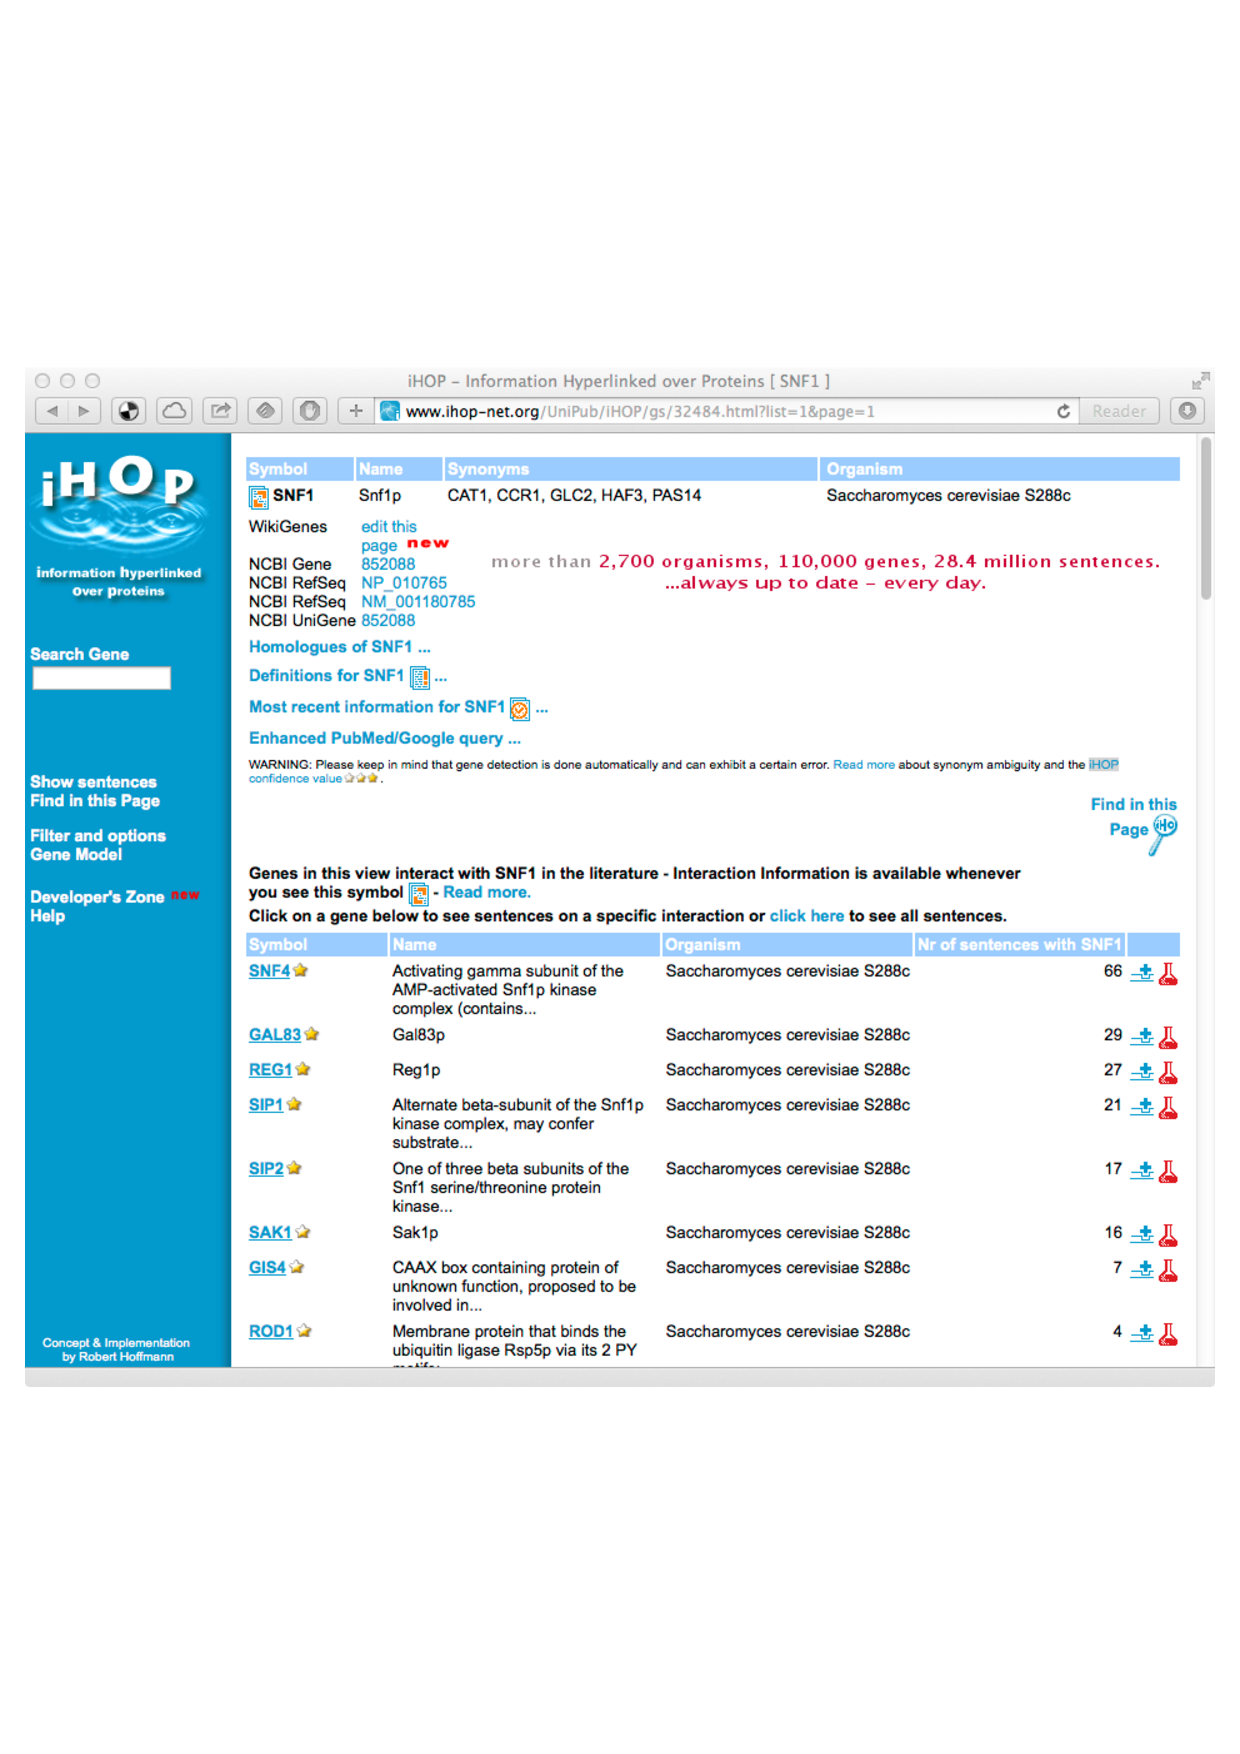
\includegraphics[scale=0.6]{figures/ihop-1.pdf}
 \caption{iHop view of interacting genes }
\label{fig:ihop-1}
\end{center}
\end{figure}    

\begin{figure}
\begin{center}
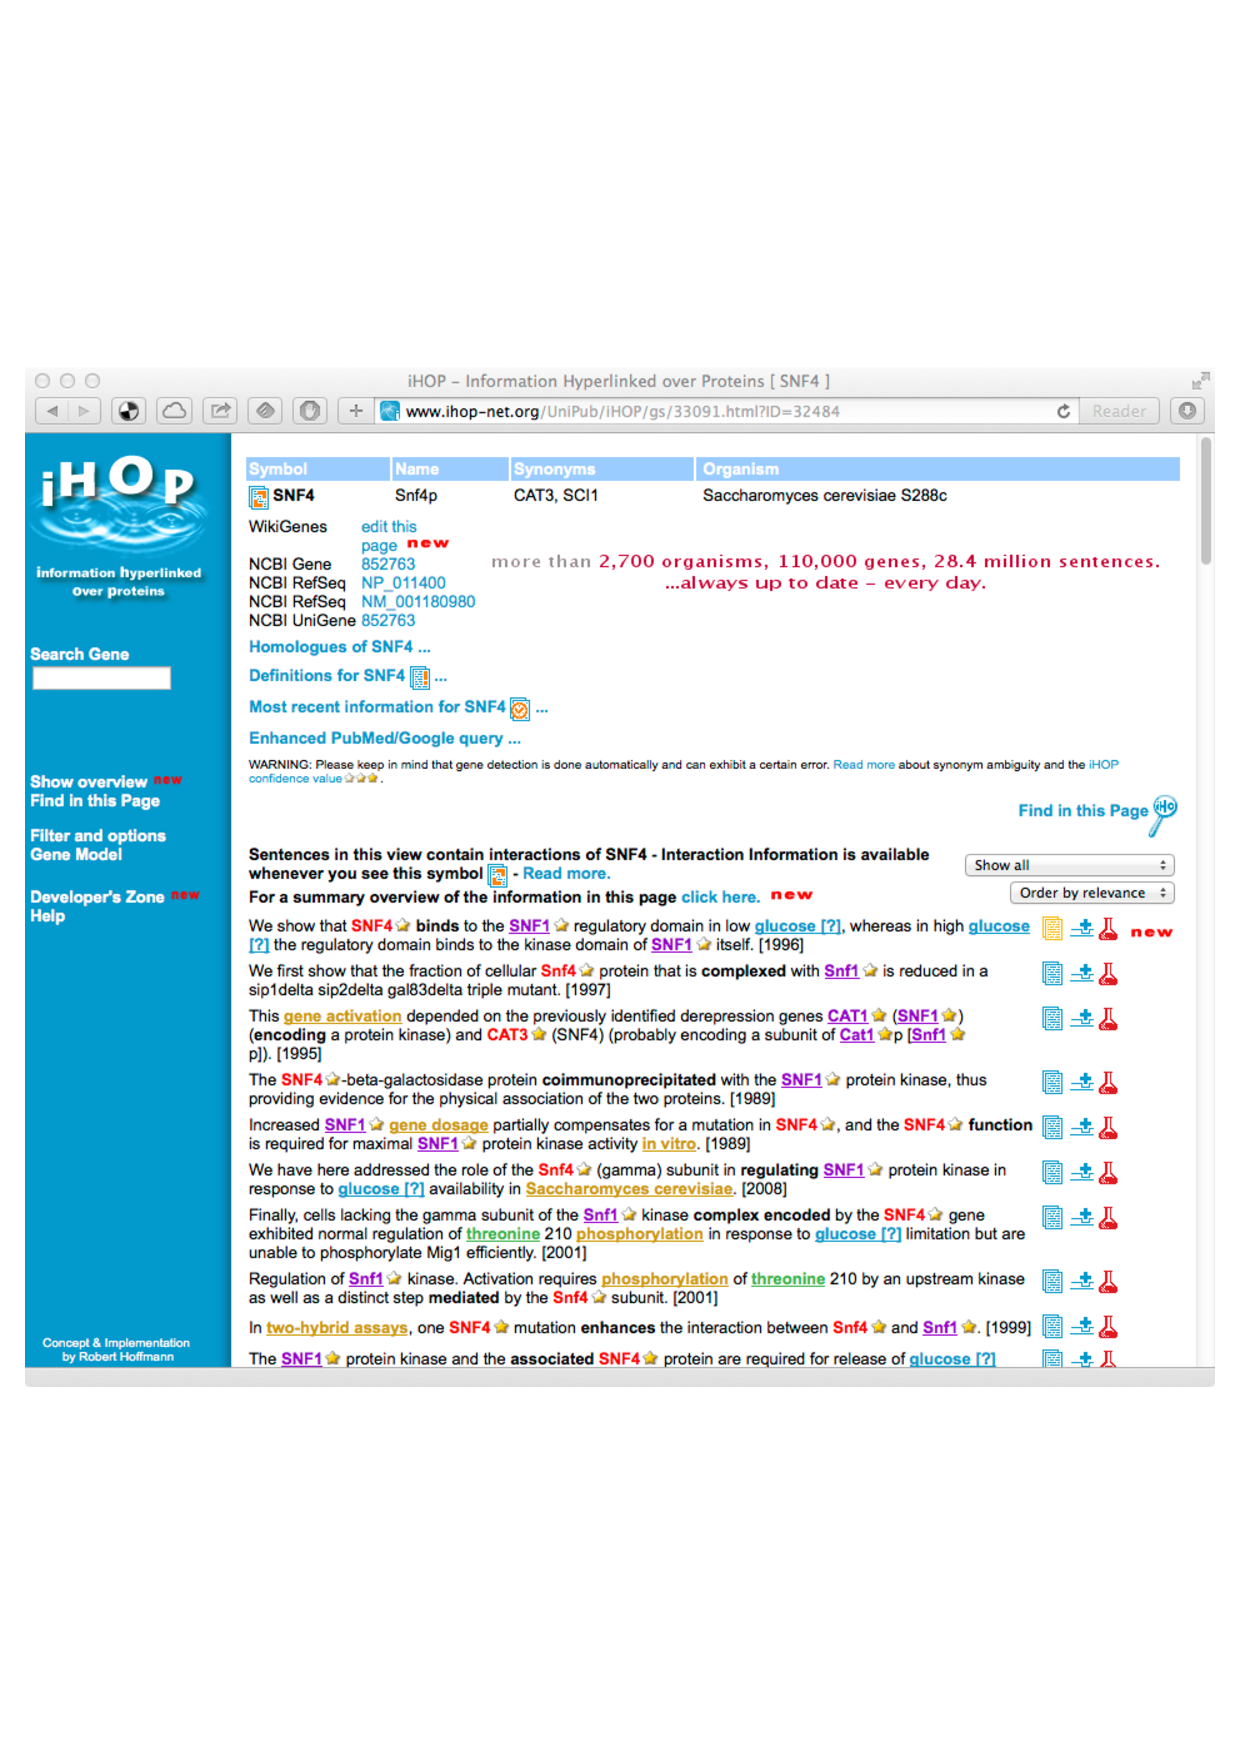
\includegraphics[scale=0.6]{figures/ihop-2.pdf}
 \caption{iHop view of sentences describing interactions}
\label{fig:ihop-2}
\end{center}
\end{figure}

\begin{figure}
\begin{center}
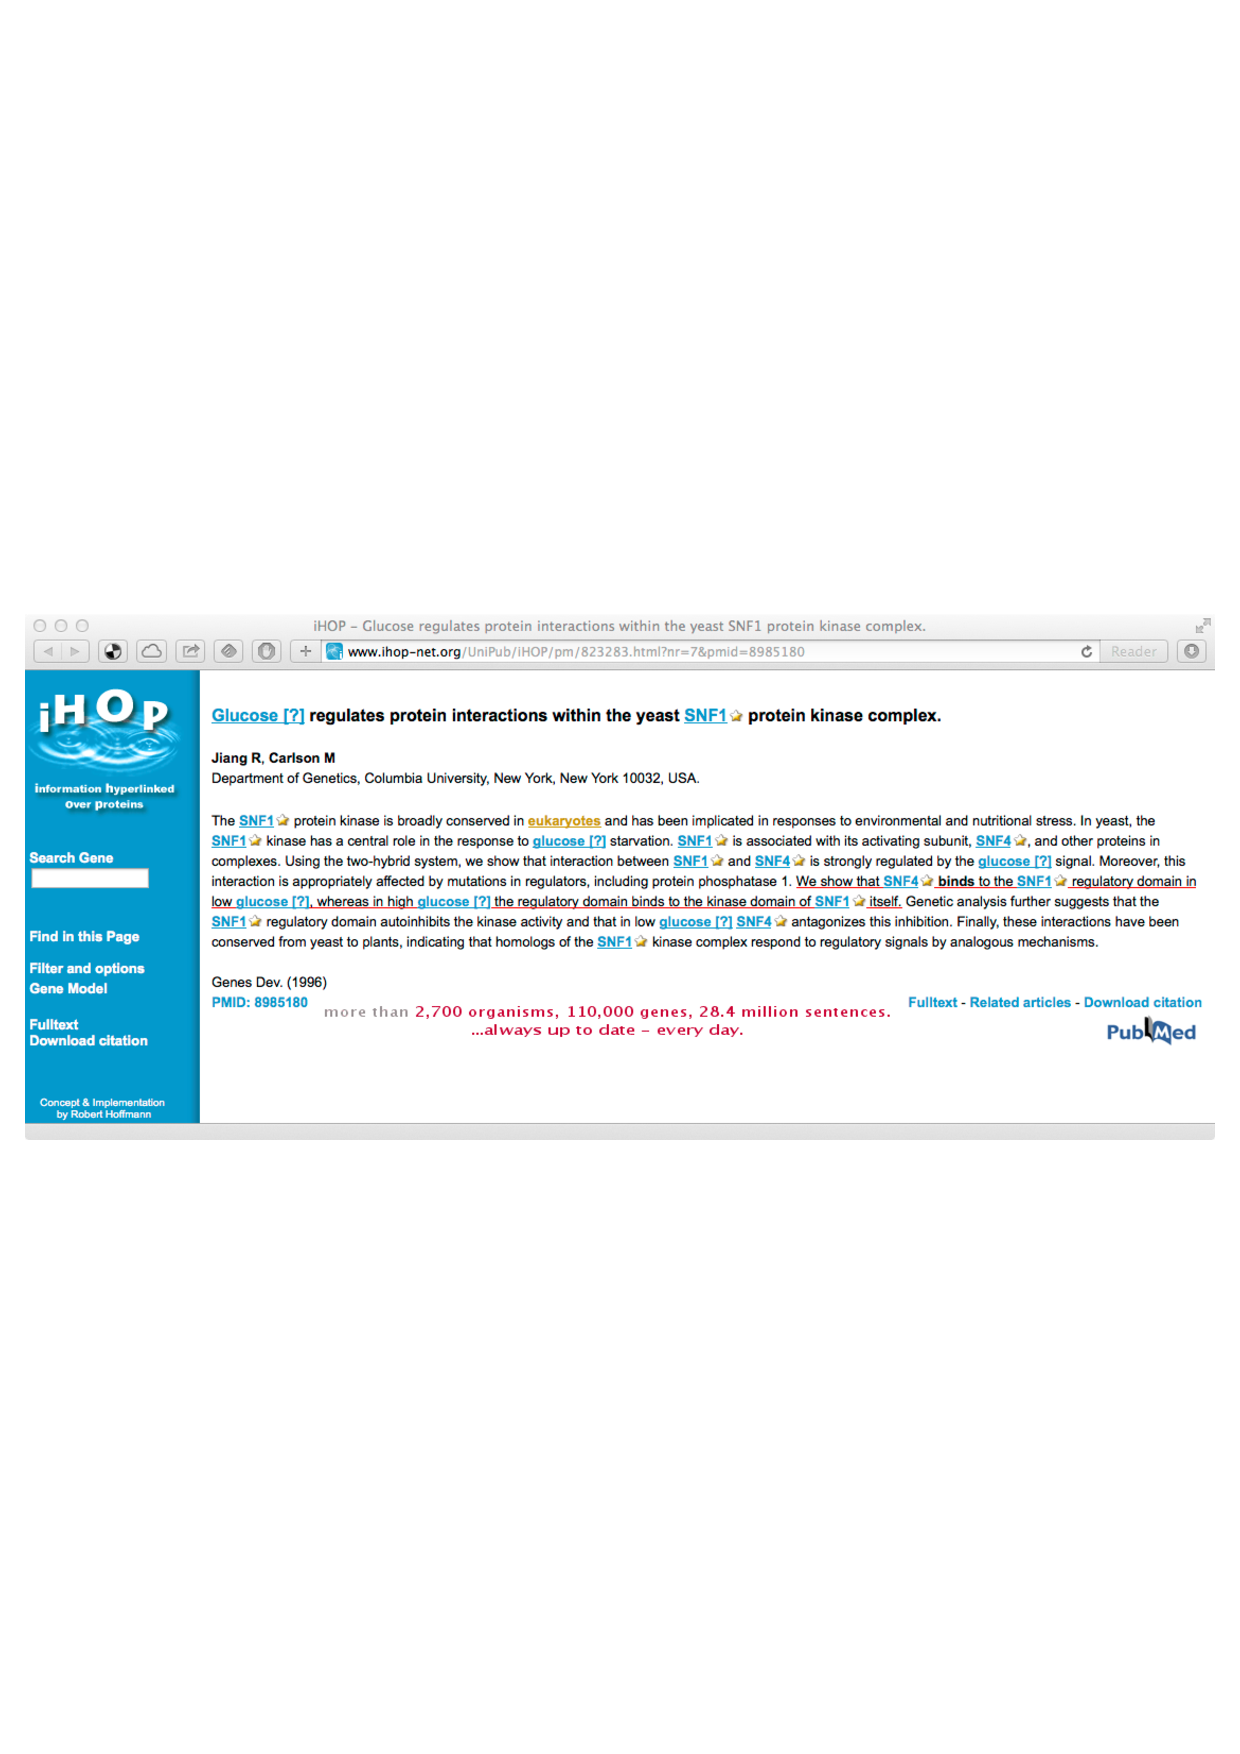
\includegraphics[scale=0.6]{figures/ihop-3.pdf}
 \caption{iHop view of hyperlinked abstract}
\label{fig:ihop-3}
\end{center}
\end{figure}

Chilibot\footnote{\url{http://www.chilibot.net}} is a similar webservice for searching PubMed abstracts \citep{Chen2004Contentrich}.
Users can search for interactions between a pairs of genes or proteins.
List of terms can be supplied to perform exhaustive searches of all possible relationships between any two terms in a list.
Search results can be further constrainted by any number of free-text keywords.
In addition, there are special keywords like \emph{modulate} that triggers a search for regulatory relationships (inhibition, stimulation, increase, reduce, etc.),  
The system returns sentences describing these interactions, linked to the abstacts they originate from.
The results are also presented as a summary graph, with nodes representing the queried terms and edges representing the relationships.

FACTA+\footnote{\url{http://www.nactem.ac.uk/facta/}} is a webservice for discovering associations between biomedical entities: gene/protein, disease, symptom, drug, enzyme, compound \citep{Tsuruoka2008FACTA}.
It indexes all abstracts in MedLine and allows users to navigate the associations and the textual evidence in an intuitive way.
Figure~\ref{fig:facta} shows FACTA+ presenting concepts associated to ``caffeine''.
Associated concepts are organized per entity class and ranked according to their association strength.
Several different measures are supported, e.g. frequency and mutual information.
Clicking on the document icon present a list of text snippets that are the source for the associations, including a link to the full abstract.
Clicking on any concept results in a new search for concepts associated to that concepts. 

In addition, it is possibly to search for indirectly related concepts through a \emph{pivot} concept.
This is akin to the ABC-linking in literature-based discovery.
Both pivot concepts and target concepts can be restricted to a certain type, for example, protein and disease.

The service has recetly been extended with a graphical visualisation component\footnote{\url{http://www.nactem.ac.uk/facta-visualizer/}}.
Figure~\ref{fig:facta-vis} shows 
This interactive visualisation also allows following links to text evidence and visualising indirect associations.

\begin{figure}
\begin{center}
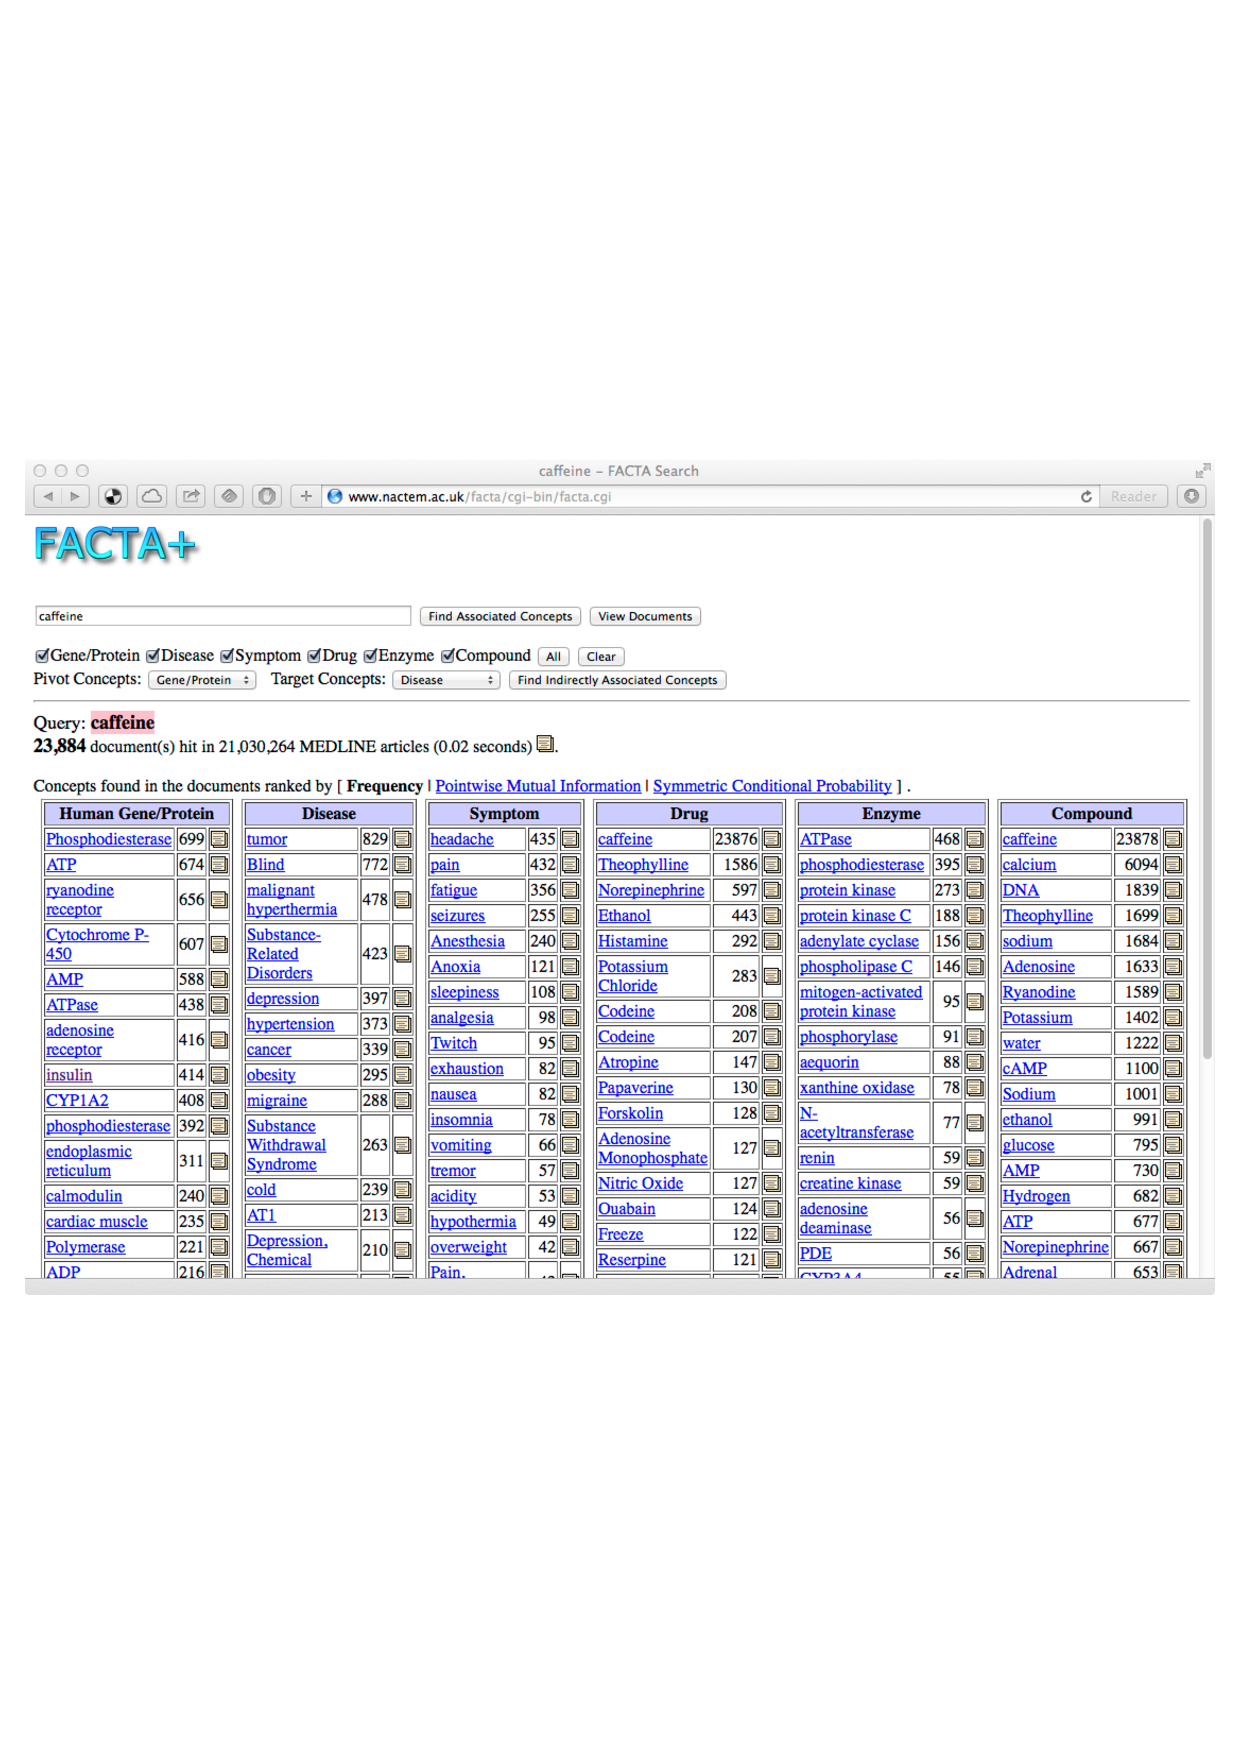
\includegraphics[scale=0.6]{figures/facta.pdf}
 \caption{FACTA+ showing concepts associated to ``caffeine'' }
\label{fig:facta}
\end{center}
\end{figure}
  
\begin{figure}
\begin{center}
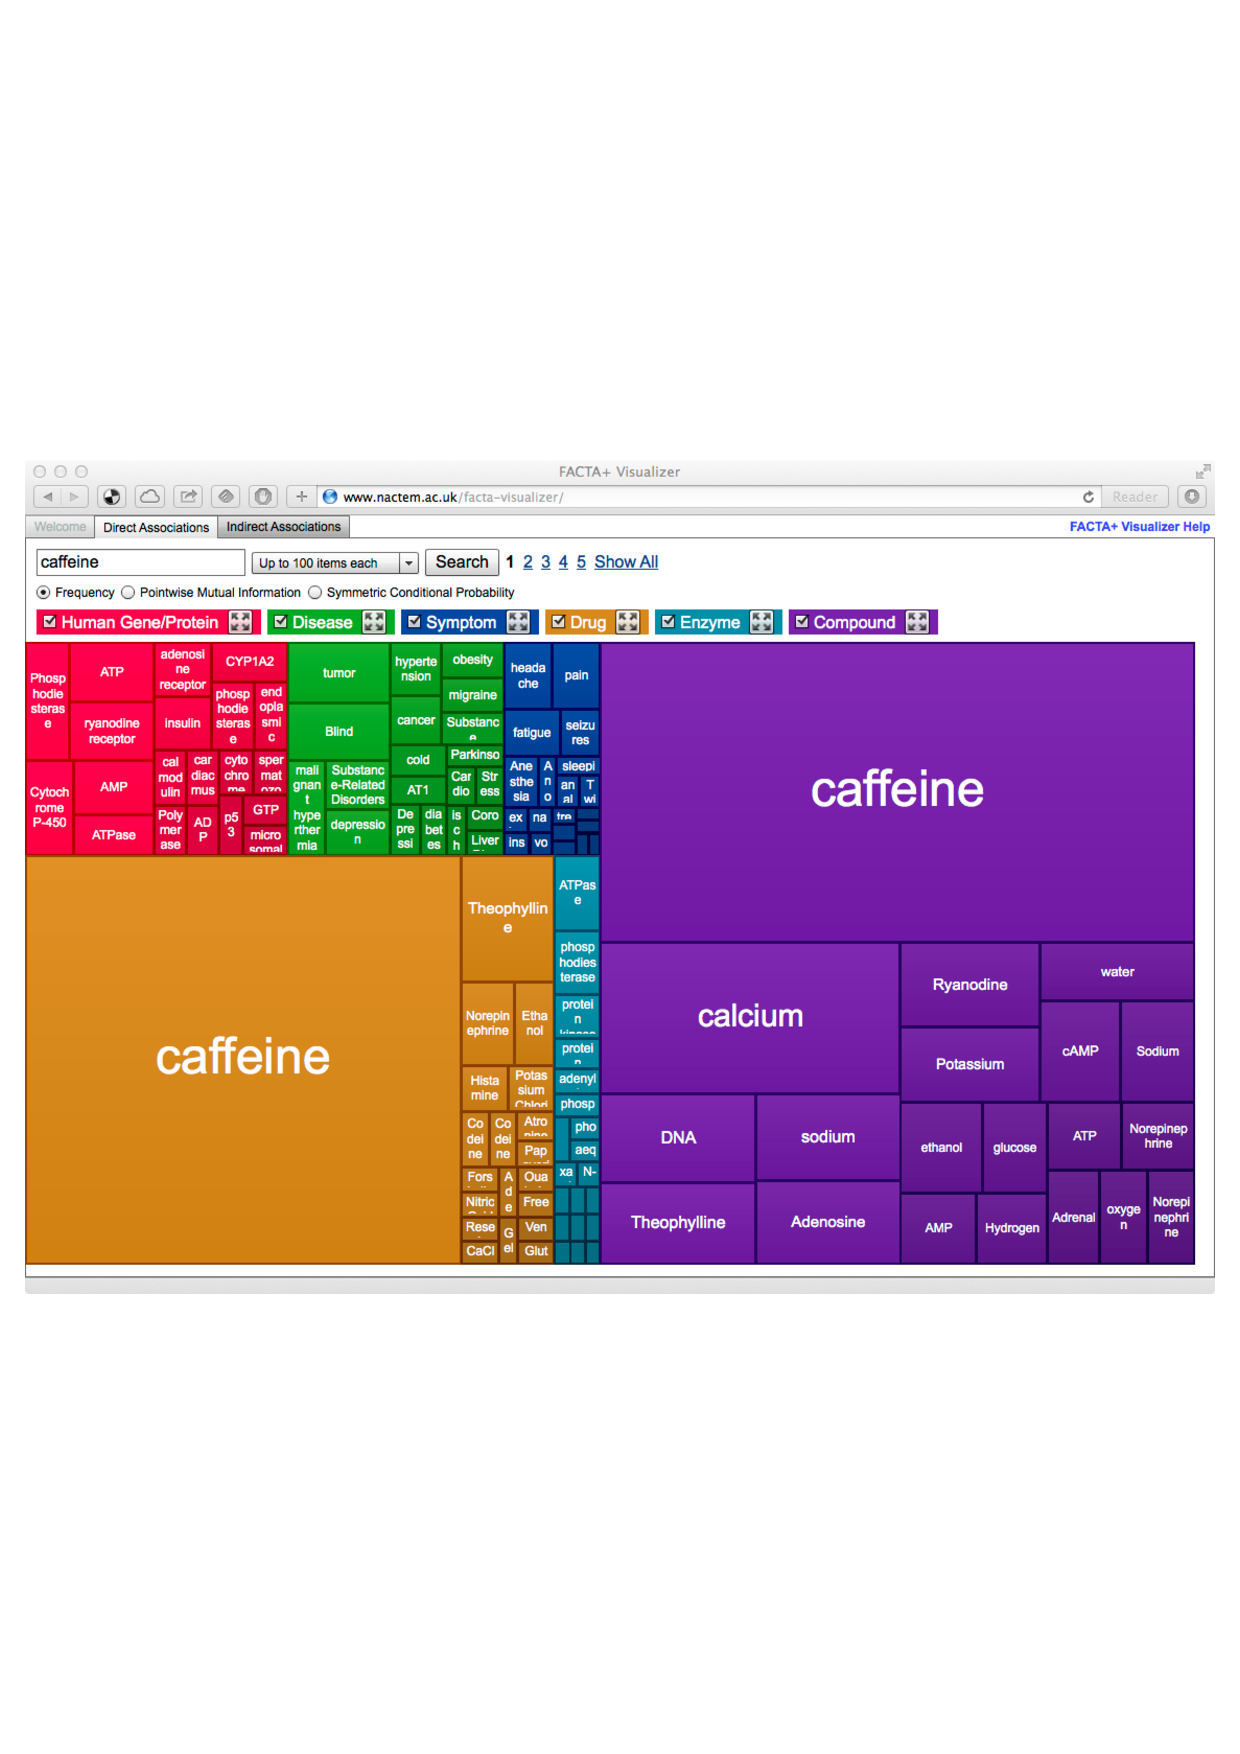
\includegraphics[scale=0.6]{figures/facta-vis.pdf}
 \caption{FACTA+ graphical visualisation showing concepts associated to ``caffeine'' }
\label{fig:facta-vis}
\end{center}
\end{figure}


\EM{More examples of applications/systems for text mining in biomedicine}


\section{Tools for Text Mining in Biomedicine}
\label{sec:tools-tm}

\subsection{Entity Detection}

\emph{Entity detection} -- often called named \emph{entity recognition} (NER) in other areas of NLP -- is the process of detecting mentions of entities in text.
Generic enitity detection tools are not well-suited for biomedical text because of highly specialized language use (jargon). 
For example, many terms have a particular meaning or do not occur at all outside of biomedical texts.
In biomedicine, it is usually quite clear what the entities of interest are, for example, genes, proteins, cells, drugs, organisms, etc.
However, detecting entities is a non-trivial task due to a number of complications.

First, there is variation in spelling and naming of entity names.
For example, a gene name may be spelled as \emph{BRCA 2},\emph{ BRCA-2},\emph{Brca2} or \emph{Brca-2} \citep{Krallinger2010Analysis}.
The use of acronyms or abbreviations instead of full names is common. 
Typos are not uncommon.
All this variation in form means that it usually does not suffice to lookup a string in a given dictionary of named entities.

Second, there is ambiguity: a term may mean different things depending on the context.
This is a common problem in NLP.
For instance, the word \emph{bat} may refer to flying animal or to a hitting instrument, depending on the context of use.
Automatically determining the right sense of a word is called \emph{word sense disambiguation}.
In biomedicine, this is often referred to as \emph{entity normalization}, where each entity mention is linked to a unique indentifier in a database, controlled vocabulary or ontology, so its meaning becomes unambiguous. 
 
Third, as science progresses in certain domain, so does the sublanguage to describe it, and consequently new terms are added all the time.
This means that systems for entity detection must be updated all the time. 
In addition, terms may gradually change meaning over time, a phenomenon known as \emph{semantic drift}.

\subsection{Relation Extraction}   

, relation extarRelation extraction aims at automatic extraction of relations between entities from text.
There is basically two approaches to relation extraction: co-occurence-based approaches and NLP-based approaches.

Co-occurence-based relation extraction follows a statistical approach. It infers that there is a relation between two entities whenever they tend to occur together frequently. 
The scope of co-occurrence can be within a fixed-sized window, a sentence, a paragraph or even a whole document. 
Different measures have been proposed to compute the association strenght between entities, but essentially all of these measure if two entities occur together more often than is to be expected by chance. 
Co-occurence-based extraction does not require any advanced NLP, so it fairly robust against e.g. very complex or ill-formed input. It tends to give high recall at the cost of low precision. 
That is, it tends to identify most of the true relations but also suggests many false relations. 
In addition, relations are non-directional, which makes the approach suitable for only certain types of relation (e.g. correlation) but unsuitable for others (e.g. causality).
NLP-based relation extraction targets binary relations such as ``protein X activates gene Y'', ``drug X treats disease Y'' or ``gene X is associated with disease Y''.
It is usually assumed that entities are already detected prior to relation extraction and that the set of targeted relations is very limited.
Still, relation extraction is a hard task because of the variation, ambiguity and vagueness in language use.
There are so many different ways to express essentially the same relation in language, that listing all of them is practically impossible: there will always be new ways to say the same thing.
Hence straight forward lookup or template matching on the word level is bound to fail.
Most systems first perform a linguistic analysis step, resulting in a more abstract representation ranging from a normalized surface string to hihh-level syntactic or semantic graph structures. 
Relations are then extracted by manually written pattern matching rules operating on these abstract representations.
Alternatively, and more popular nowadays, extraction is performed in a data-driven fashion, where supervised machine learning algorithms learn to recognize relations from training examples.
This requires an annotated corpus of text material in which relations are labeled by human annotators.
NLP-based extraction systems are more brittle, because they depend very much on the quality of the NLP tools such as part-of-speech taggers and syntactic parsers.
They tends to give high precision but low recall.
They are also more expensive to build, because of manual labour involved in writing pattern matching rules or annotating training corpora.
However, extracted relations can be directional, which makes them potentially more useful for many applications. 

Hybrid systems combine different approaches, sometimes both co-occurence-based and NLP-based, to obtain better performance.
Another recent trend is to perform entitity recognition and relation extraction simultaneously in a single unified system.
This potentially avoids error propagation in cases where failure to detect the correct entities prevents extraction of the correct relation.
  
\subsection{Event Extraction}

Event extraction may be regarded as a generalization of relation extraction.
Where relation extraction is limited to binary relations between two entities, events can involve multiple entities.
These are labeled according to the role they play in the event, often called \emph{thematic roles}.
Moreover, one event can play the role in another event, giving rise to recursive structures.
Figure~\ref{fig:event-example} shows an example of an event from the BioNLP event extraction task.
It has an event called \emph{Phosphorylation} that applies to the protein STAT3, which therefore plays the role of \emph{Theme} in this event.
This \emph{Phosphorylation} event in turn plays the role of \emph{Theme} in another event called \emph{Regulation}, which also involves the protein Vav in the role of \emph{Cause}.
A third event takes the same \emph{Theme} role (\emph{Phosphorylation}) but a different \emph{Cause} (Rac-1).

\begin{figure}
\begin{center}
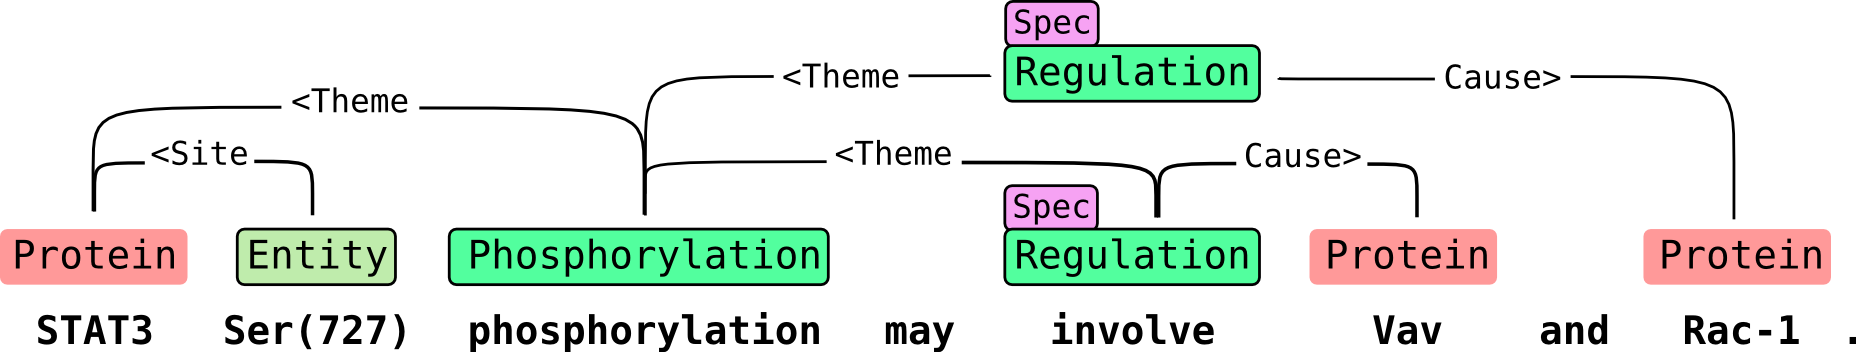
\includegraphics[scale=0.65]{figures/event-example.png}
 \caption{Example of an event from the BioNLP event extraction task \citep{Bjorne2011EXTRACTING}}
\label{fig:event-example}
\end{center}
\end{figure}

Event extraction are almost exclusively NLP-based and usually involve syntactic parsing.
It is closely related to the task of \emph{semantic role labelling} (SRL) which aims to label predicates and their semantic roles according to some general linguistic theory about semantic frames. 
Approaches can be knowledge-based (hand-written rules), data-driven (supervised machine learning) or hybrid.
Probabably the most succesful event extraction system for biomedicine acording to recent system evaluations is the Turku Event Extraction Systeem (TEES), which is a machine learning system employing support vector machines in combination with separate systems for entitity detection and syntactic parsing \citep{Bjorne2011EXTRACTING}. 

Recently particular aspects of events have extracted attention, for example, negation and speculation. Negation detection systems try to detect if an event is in the scope of a of negation -- e.g. \emph{not}, \emph{neither} or \emph{lack of evidence for}. 
Evidently, knowing that a fact is negated is crucial in any text mining application.
Likewise, detection of speculation, modality, uncertainty or hedging provides important information.
For example, an event may be qualified as \emph{possible}, \emph{unlikely} or \emph{not always}.
The two regulation events in Figure~\ref{fig:event-example} are marked as \emph{Spec} (speculative) because of the modal verb \emph{may}, which signals a certain amount of uncertainty.

\subsection{Evaluation}

Comparing different approaches proposed to entity detection, relation extraction, event extraction and similar tasks in information extration and text mining is not easy, because results reported in the literature on different text material, or using different evaluation methods and measures, can not be compared with each other.
However, without proper empirical evaluation, it is essentialy impossible to judge if any progress is made.
Several evaluation initiatives in biomedical NLP and text mining have addressed this issue, including the BioCreative and BioNLP shared tasks.
These follow the established practice in NLP and machine learning of providing a standard evaluation framework for a particular task consisting of labeled development data, blind test data and proper evaluation measures.   
Participants build systems for performing the task -- e.g. entity detection -- on the basis of the labeled development data.
They then apply their systems to label the the blind test data.
The shared task organisers compare the system predictions to the true answers (gold standard) according to some evaluation measures, which allows the different systems to be ranked according to their performance on the task.
Systematic comparison of the performance of different methods, in combination with detailed error analysis, defines the state-of-the-art and suggests ways for further improvement.

Although this methodology has been instrumental in progressing the field, it is not without its disadvantages.
For instance, systems are known to become overfitted on the type of text used in the evaluation.
Applying the same system to text from a different domain may lead to dramatic drops in performance. 

\section{Machine Reading and Open Information Extraction}

There are two other areas which are closely related to text mining, both involving NLP.
The idea of \emph{machine reading} is essentially to enable computers to read text in electronic format, understand its meaning and extract knowledge from it in the same way as humans do \citep{Mitchell2005Reading}.
Given the enormous amount of computer-readable text available on the internet and from scanned books, a functional machine reading system would allow computational agents to acquire knowledge on an unprecedented scale.
\emph{Open information extraction} also aims for knowledge base population through informatin extraction from text \citet{banko2007open,Etzioni2011Search}.
In contrast to traditional information extraction, where there is a fixed set predetermined relations, in open IE the set of relations is open, that is, any relation encoded in text is targeted.  
Examples include the TextRunner open IE system and its succesors \citep{yates2007textrunner}, the DeepDive system \citep{niu2012deepdive}, CMU's Never Ending Language Learner (NELL) \citep{carlson-aaai} that learns to extract facts from the webpages,  MPI's YAGO system that learns fact from Wikipedia and combines them with WordNet \citep{YAGO} and IBM's Watson system that played Jeopardy \citep{fan2012automatic}.

\todo[inline]{inference and reasoning, relation to GOFAI}


%%% Local Variables: 
%%% mode: latex
%%% TeX-master: "ocwp1-d1"
%%% End: 

 

\chapter{Literature-based Knowledge Discovery}

\todo[inline]{key publications, approaches, software and resources on Literature-Based Knowledge Discovery}

\chapter{Text mining in Climate, Marine and Environmental Science}

\todo[inline]{Text mining work in related areas, e.g. Kyoto, GeoDeepDive, text mining for Marine Ecological Genomics, environmental QA in machine reading challenge}

Text mining of scientific literature, and literature-based knowledge discovery in particular, has its roots in biomedicine.
Research has matured to a level that text mining applications and services have started to be really helpful to researchers in biomedicine.
Although biomedicine is still by far the most popular application domain, literature mining is now gradually spreading out to other scientific fields.
Yet, despite our best efforts in searching the literature, published work on text mining in climate, marine or environmental science turned out to be extremely rare.
On the one hand, this is unfortunate, because it means there is almost no prior work in our domain of interest that we can build on.
On the other hand, it indicates that the work on literature-based discovery in Ocean-Certain is pushing the limits and holds potential for delivering new and interesting results.

Given the lack of prior art, this chapter surveys work in fields outside biomedicine but related to Ocean-Certain, in fields such as chemistry, geology and ecology.
The first part describes tools and resources, whereas the second part addresses complete systems. 

\section{Tools and Resources}

\subsection{Vocabularies , Taxonomies and Ontologies}

There are several specialised controlled vocabularies and ontologies which may benefit text mining in climate, marine and environmental science.
 
The Environment Ontology\footnote{\url{http://environmentontology.org/home}} (EnvO) is an ontology about environments  \citep{Buttigieg2013Environment} of biological organisms.
It provides a controlled, structured vocabulary of over 1800 terms to annotate biological entities or samples with environmental descriptors.
There are three main types of terms:

\begin{itemize}
\item \emph{biome}: e.g., boreal moist forest biome, tropical rain forest biome, and oceanic pelagic zone biome 
\item \emph{environmental feature}: e.g, mountain, pond, whale fall, and karst
\item \emph{environmental material}: e.g., sediment, soil, water, and air
\end{itemize}

\noindent The ontology is intended to facilitate integration, archiving and federated searching of environmental data.
It also contains environmental terms in the domain marine biology.
For example, Figure~\ref{fig:envo-example} shows the term \emph{marine algal bloom}.
The left side shows a definition, known synonyms (\emph{red tide}), and links to external definitions like the one in Wikipedia.
The right side shows a graphical representation of the ontological relations.
For instance, that \emph{marine algal bloom} is a kind of \emph{algal bloom}, which ultimately is a kind of \emph{environmental feature}, and that  \emph{marine algal bloom} is located in a\emph{ marine biome}, which ultimately is an \emph{environmental system.}

\begin{figure}
\begin{center}
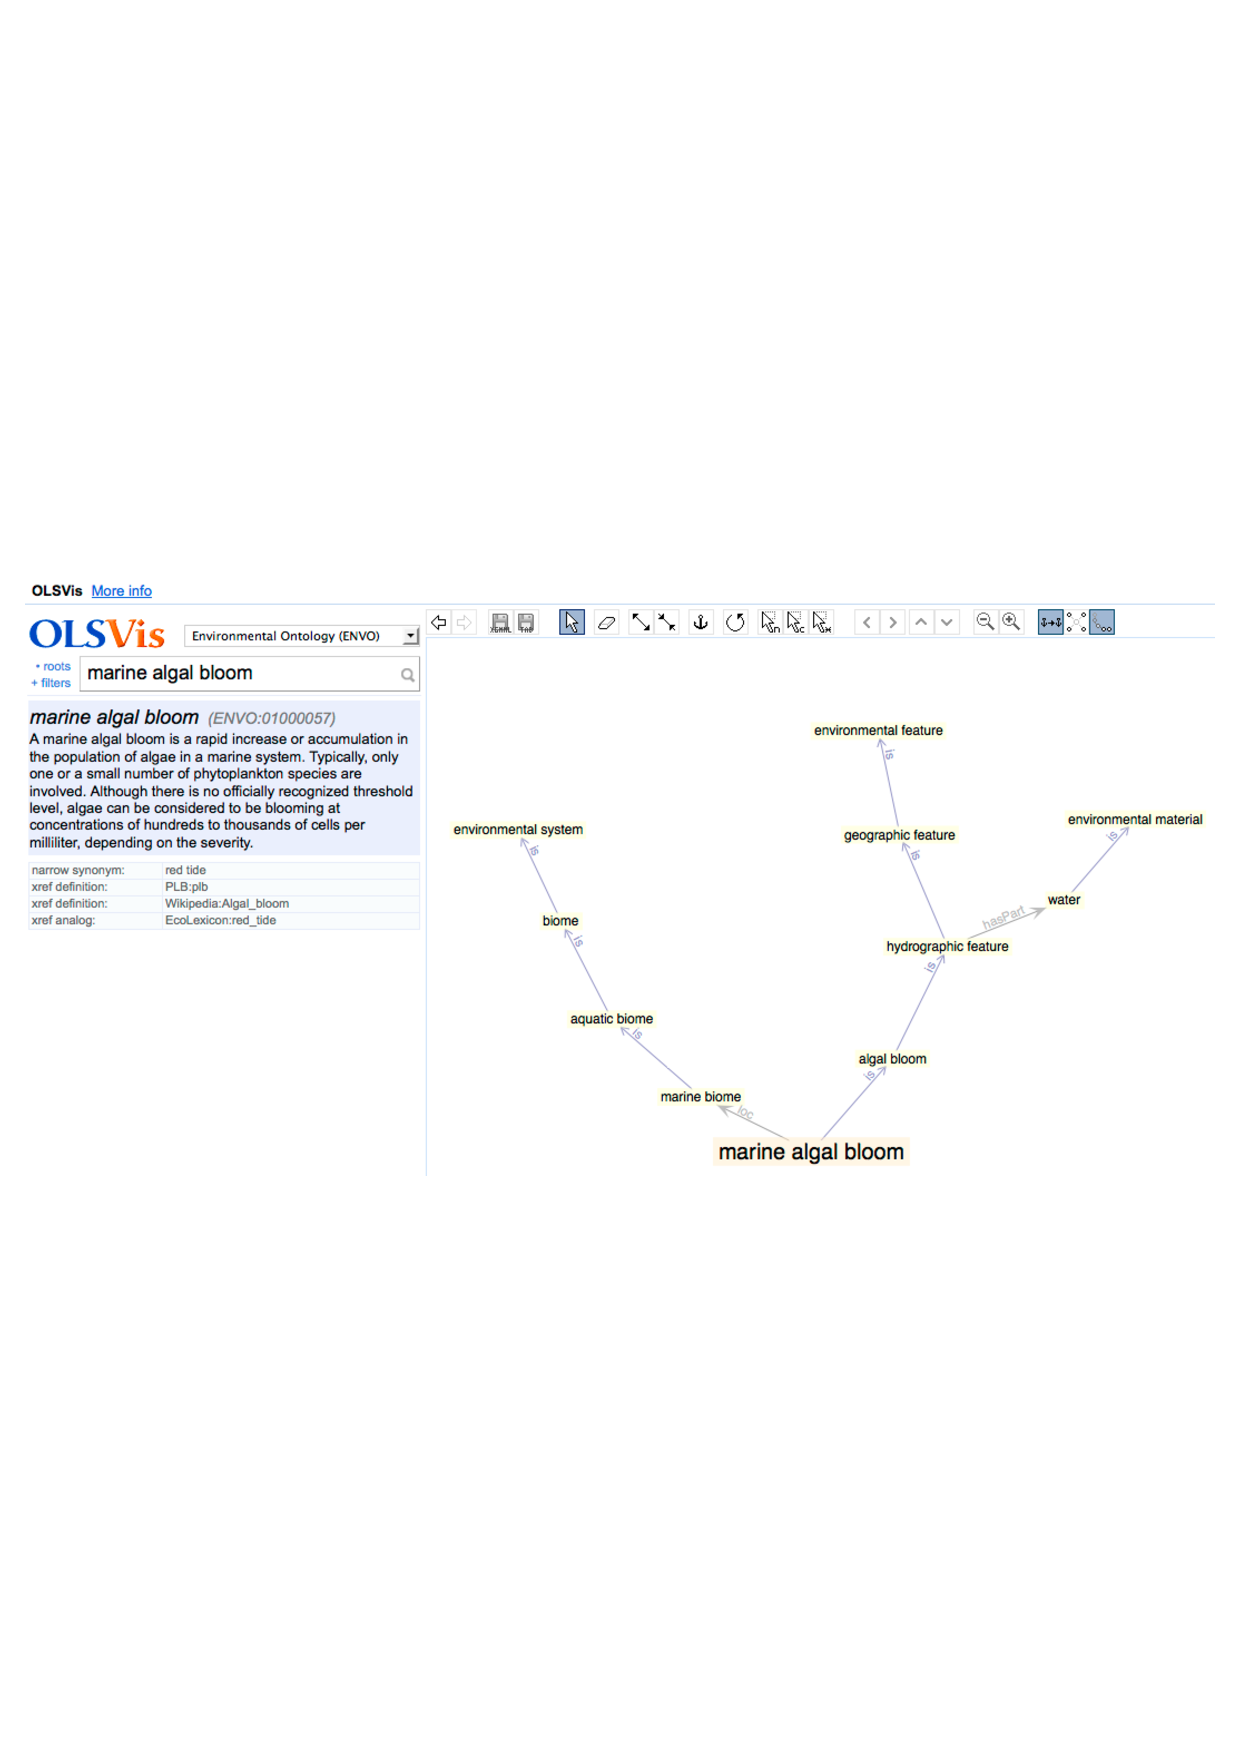
\includegraphics[scale=0.6]{figures/envo-example.pdf}
 \caption{Example of entity \emph{marine algal bloom} in EnvO ontology}
\label{fig:envo-example}
\end{center}
\end{figure}


WoRMS\footnote{\url{http://www.marinespecies.org/}}  (World Register of Marine Species) aims to provide an authoritative and comprehensive list of names of marine organisms, including information on synonymy \citep{Costello2013Global}.
It contains over 220 thousand species, with an estimated coverage of over 95\%.
There is a web service for tasks such getting the full classification for your taxa, resolving unaccepted names to accepted ones or resolving a common name to a scientific name.

The Marine Metadata Interoperability\footnote{\url{https://marinemetadata.org/}} (MMI) project has as its mission promoting the exchange, integration and use of marine data through enhanced data publishing, discovery, documentation and accessibility.
It hosts, among other things, an ontology repository and associated semantic framework that can be used by the marine science community to store, manage, and work with its scientific vocabularies.

\subsection{Named Entity Taggers}

Many named entity taggers are developed for biomedicine and target specific entities of interest in this domain, such a proteins, genes and drugs.
These are of limited use for text mining in climate, marine and environmental science. 
However, there are a number of taggers for recognition and normalisation of biological or chemical entities that are potentially useful for our purposes.

LINNAEUS\footnote{\url{http://linnaeus.sourceforge.net/}} is an open-source software package for species name recognition and normalisation \citep{Gerner2010LINNAEUS}. 
Entities are normalised by linking them to unique identifiers the NCBI taxonomy database\footnote{\url{http://www.ncbi.nlm.nih.gov/taxonomy}}, a curated classification and nomenclature for all of the organisms in the public sequence databases, covering about 10\% of the described species of life on the planet.
It uses a dictionary-based approach to identify species names and a set of heuristics to resolve ambiguous mentions, obtaining 94\% recall and 97\% precision on entity recognition, with 97\% of all mentions resolved to the correct NCBI taxonomy identifiers.
 
The SPECIES (Identification of Taxonomic Mentions in Text) project\footnote{\url{http://species.jensenlab.org/}} has developed taggers for species and organism mentions in text \citep{Pafilis2013SPECIES}. 
The taggers allow for both identification of names in the text and normalisation to the corresponding entries in the NCBI taxonomy.
These tools are claimed to be an order of magnitude faster than LINNAEUS.

OSCAR4\footnote{\url{https://bitbucket.org/wwmm/oscar4}} (Open Source Chemistry Analysis Routines) is an open source extensible system for the automated annotation of chemistry in scientific articles \citep{Jessop2011OSCAR4}.
It can be used to identify chemical names, reaction names, ontology terms, enzymes and chemical prefixes and adjectives, and chemical data such as state, yield, IR, NMR and mass spectra and elemental analyses. 
In addition, where possible, any chemical names detected will be annotated with structures derived either by lookup, or name-to-structure parsing using OPSIN or with identifiers from the ChEBI (Chemical Entities of Biological Interest) ontology.

ChemSpot\footnote{\url{https://www.informatik.hu-berlin.de/forschung/gebiete/wbi/resources/chemspot/chemspot/}} is another set of tools for named entity recognition and classification of chemicals in texts, including trivial names, abbreviations, molecular formulas and International Union of Pure and Applied Chemistry (IUPAC) chemical compounds. 
ChemSpot employs supervised-machine learning (Conditional Random Fields) and a dictionary, as well as pattern-based recognition, a classifier model and several methods for consolidating all annotations. 
ChemSpot also performs entity normalisation by assigning identifiers from numerous chemical databases. 

CheNER\footnote{\url{http://chener.bioinfo.cnio.es/}} (Chemical Named Entity Recognizer) is another recent tool. It specialises in processing IUPAC entities, on which it is shown to outperform Chemspot \citep{Usie2014CheNER}.

The ENVIRONMENTS\footnote{\url{http://envo.her.hcmr.gr/environments.html}} (Identification of Environment Descriptive Terms in Text) project aims to produce software identifying environment descriptive terms in text, such as \emph{coral reef}, \emph{cultivated land}, \emph{glacier}, \emph{pelagic}, \emph{forest} or \emph{lagoon}.
It allows for orthographic variation in the way the terms are written (e.g. plural forms and spacing/hyphenation like in freshwater, fresh-water, and "fresh water).
Terms are normalised by linking them to a unique identifier is the Environmental Ontology (EnvO).
The project is ongoing and as of yet no software has been released.

\section{Text Mining Systems}

EnvMine is a text-mining system in the field of microbial ecology that automatically extracts contextual information from text like published articles or web pages \cite{Tamames2010EnvMine}.
The motivation is that in ecological studies, it is crucial to have adequate descriptions of the environments and samples being studied. 
Two types of contextual information about sampling sites are targeted: physicochemical variables and geographical locations.
Physicochemical variables include temperature, size, volume, pH, concentration, time, weight, area, pressure and salinity.
These are expressed by a combination of measure and unit, e.g. ``a depth of 250 ''.
As often the variable is implicit in the text, the system is capable of inferring it; e.g. it infers from ``5 degrees C'' that the variable is ``temperature''.  
Geographical locations are normalised by geographical coordinates. 
The system is quite accurate, achieving a recall of 92\% with less than 1\% error on variables, whereas it achieves 86\% recall with 92\% precision on geographical locations.

Related to this is the shared task on bacteria biotope at BioNLP 2011 and 2013 \citep{bossy2013bionlp}.
The bacteria biotope task is to extract bacteria and their locations from scientific web pages and to characterise these locations with respect to the OntoBiotope ontology of microbe habitats.
This facilitates studying the interaction between species and their environment and  the underlying biological mechanisms at a molecular level.
There are two sub-tasks, entity detection and event extraction.
An example of event extraction is shown in Figure~\ref{fig:biotope}.
\emph{Localisation} relations link bacteria to the place where they live, e.g. \emph{Bifidobacterium longum} to \emph{adult humans}.
\emph{PartOf} relations link habitat entities to their parts, e.g. \emph{adult humans} to \emph{gut}.
There were four participating systems in the 2013 task, with F-scores ranging from 0.44 to 0.61 on entity detection and scores from 0.27 to 0.6 on event extraction, indicating that the tasks are challenging. 

\begin{figure}
\begin{center}
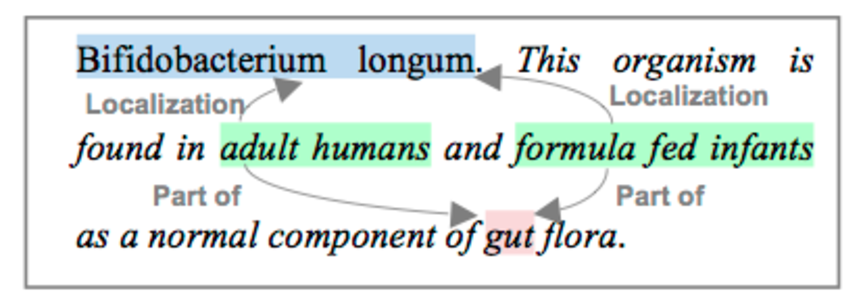
\includegraphics[scale=0.6]{figures/biotope.pdf}
 \caption{Example of event extraction task in BioNLP 2013 task on bacteria biotope \citep{bossy2013bionlp}}
\label{fig:biotope}
\end{center}
\end{figure} 

The KYOTO\footnote{\url{http://kyoto-project.eu/}} (Knowledge Yielding Ontologies for Transition-based Organizations) project developed a system that allows people in communities to define the meaning of their words and terms in a shared Wiki platform in a formal way \citep{Vossen2008}.
Part of the project was developing tools to automatically extract facts from large amounts of text and making these fact bases available.
One of the application domains was environmental science.
Figure~\ref{fig:kyoto} shows a graph representing facts extracted from a single sentence.
Several large sets of extracted facts can be downloaded, including those from publications by European Environment Agency and articles from the Journal of Environmental Biology.\EM{Kyoto deserves much more attention, but the website is such a mess that is hard to figure out the big picture.}  

\begin{figure}
\begin{center}
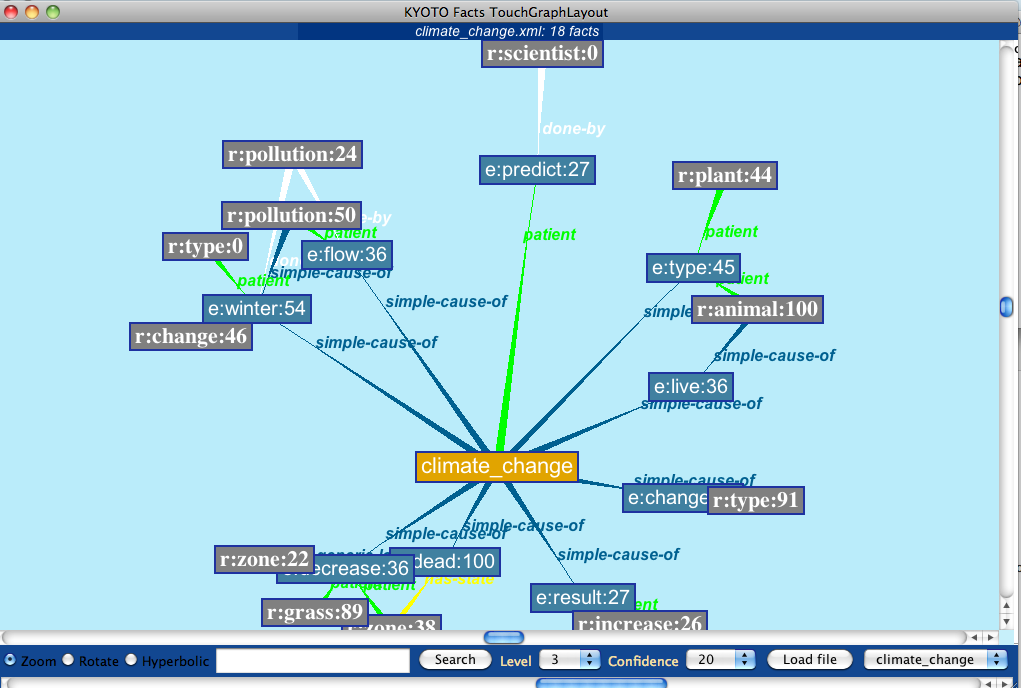
\includegraphics[scale=0.35]{figures/kyoto.png}
 \caption{Fact graph extracted by Kyoto system from the sentence ``Scientists predict that climate change could also cause a decrease in underwater grasses, more "dead zones" of low oxygen, more annual precipitation and a resulting increase in the flow of pollution, fewer wintering waterfowl, and a change in the types of plants and animals that live in the area.''}
\label{fig:kyoto}
\end{center}
\end{figure} 


GeoDeepDive\footnote{\url{http://hazy.cs.wisc.edu/hazy/geodeepdive}} is another text mining system for extracting information and knowledge from text, tables, and figures of geology journal articles \citep{Zhang2013GeoDeepDive}.
It combines data from several sources: unstructured data (html documents, scanned papers, images), structured knowledge bases (Freebase, dictionaries), domain experts (expert rules and annotation) and crowds (annotation).
It performs extraction of entities (e.g., rock formations, locations, temporal intervals, etc.) and relations.
The goal is to support novel geological science, e.g., understanding the carbon cycle and characterising the organic carbon content of Earth’s crust.
Figure~\ref{fig:geodeepdive} shows two examples of the user interface.
The top half shows a geographical representation of sample extraction throughout Northern America, where polygons represents a geological areas and their opacity indicates the number of extractions in that area.
The right hand side shows statistics such as total the number of units and measurements extracted from 36162 documents.
The bottom figure shows extractions for a particular rock formation (Barnett).
A table with measurements for Total Organic Carbon (TOC) is shown, together with the provenance, i.e. a the source text for the extraction.
Users are asked to provide feedback regarding the correctness of the extracted data, which is then used to improve the system.

A related project called PaleoDeepDive\footnote{\url{http://youtu.be/Cj2-dQ2nwoY}} has been started very recently.
It extracts fossil data -- such as biological classification, geographical distribution and geological location -- from journal articles and books on paleobiology.
One the aims is producing a more reliable biodiversity curve, which represents variation in the overall number of species over the past million of years.

\begin{figure}
\begin{center}
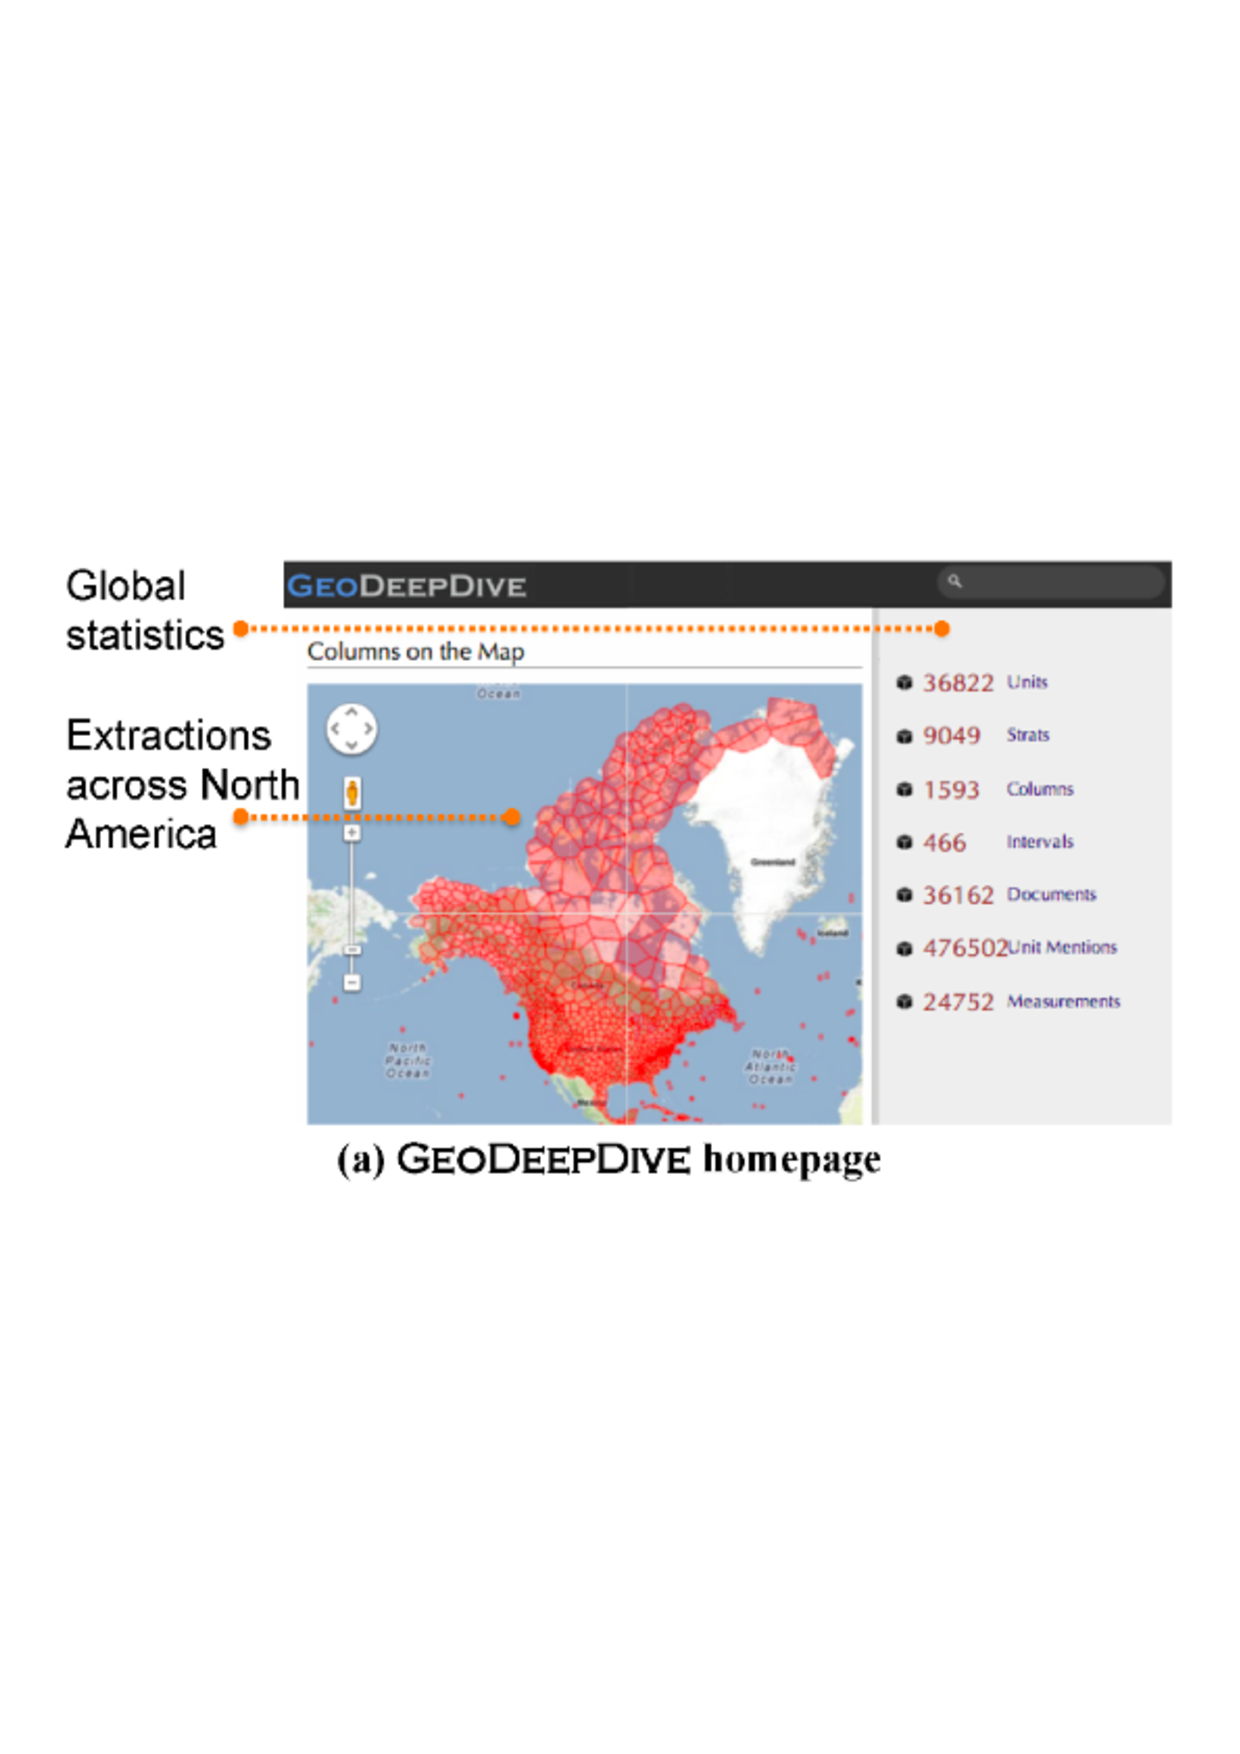
\includegraphics[scale=0.6]{figures/geodeepdive-1.pdf}
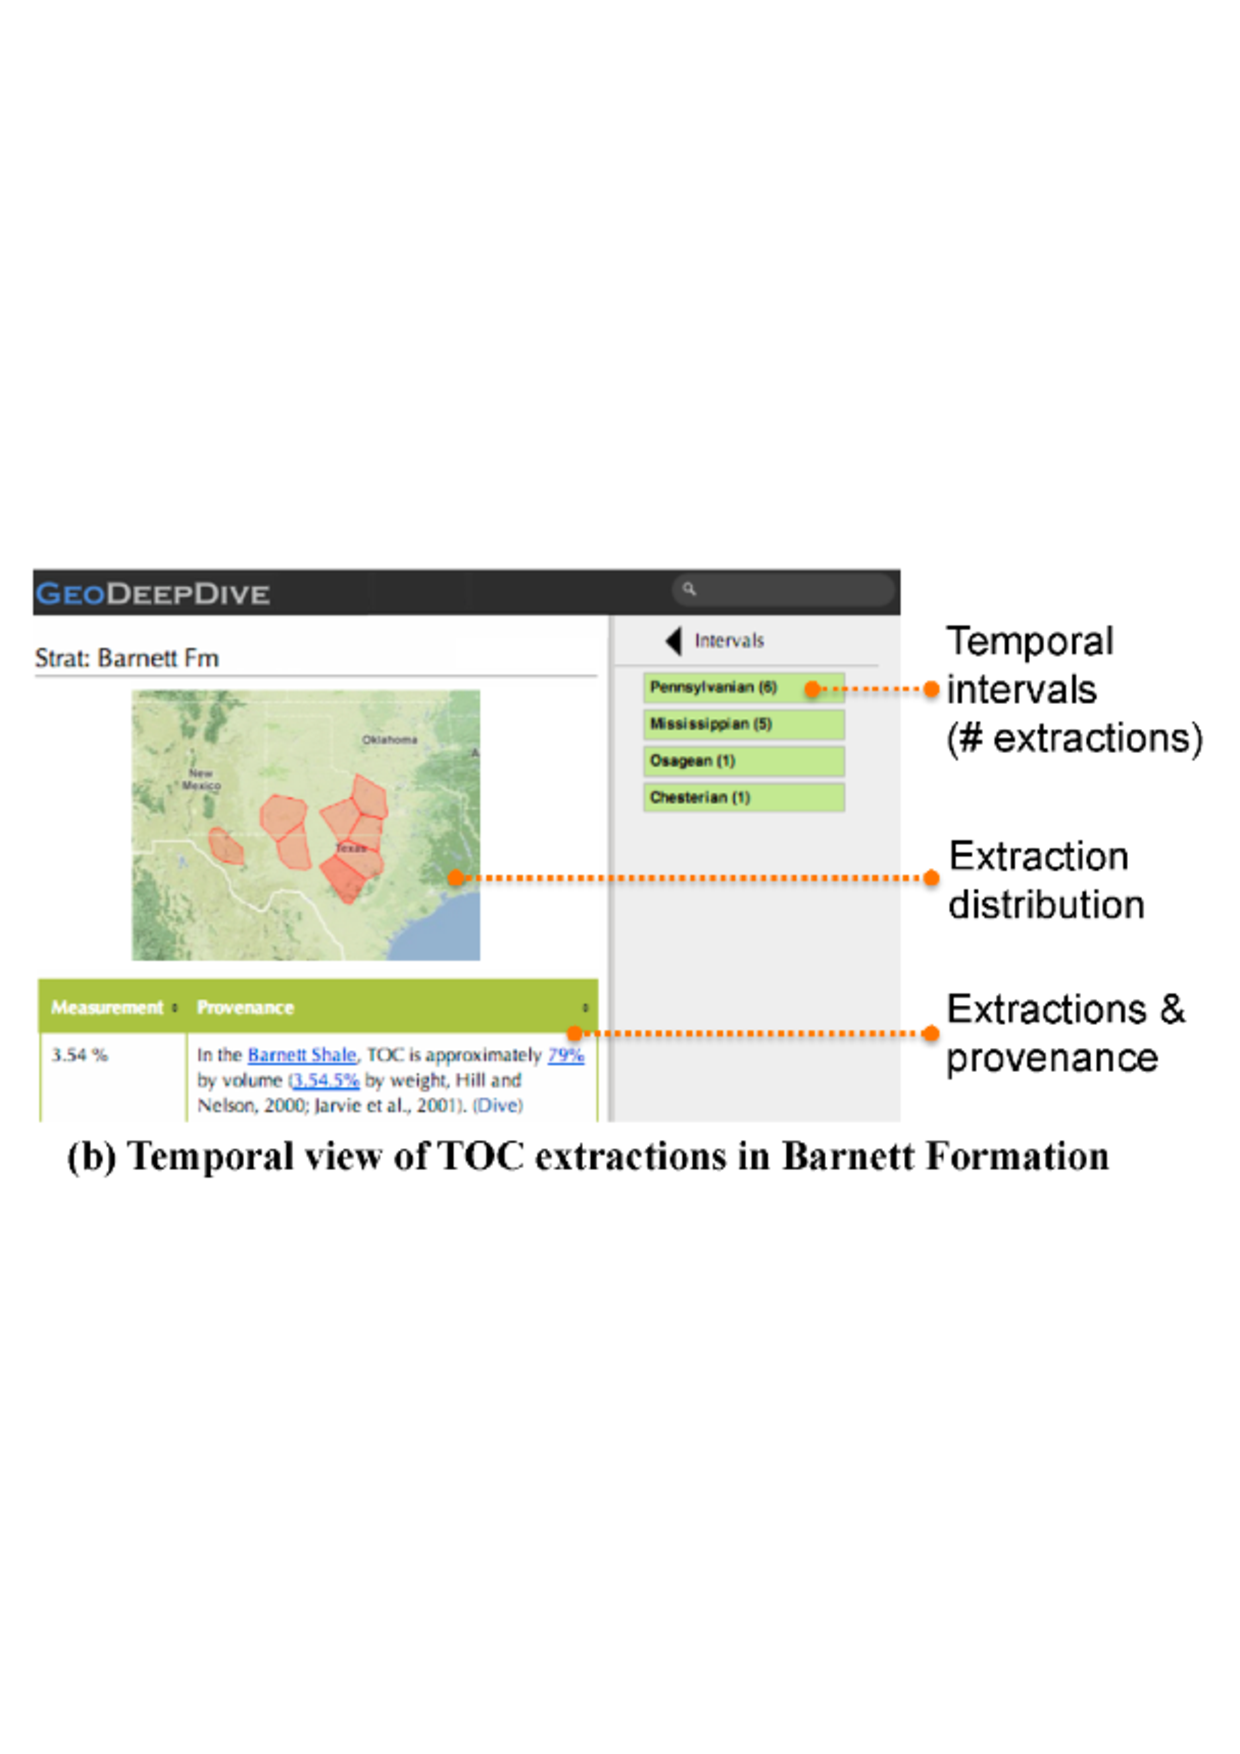
\includegraphics[scale=0.6]{figures/geodeepdive-2.pdf}
 \caption{GeoDeepDive user interface \citep{Zhang2013GeoDeepDive}}
\label{fig:geodeepdive}
\end{center}
\end{figure} 
   
In the area of ocean management, \citet{Ekstrom2008Exploratory} describe exploratory text mining of ocean law to measure overlapping jurisdictions of government agencies.  


%%% Local Variables: 
%%% mode: latex
%%% TeX-master: "ocwp1-d1"
%%% End: 

%
\chapter{Ongoing and future work} 

\todo[inline]{Brief description of our current work and plans on LBD}


%%% Local Variables: 
%%% mode: latex
%%% TeX-master: "ocwp1-d1"
%%% End: 


\bibliographystyle{plainnat}
\bibliography{ocwp1_d1}

\end{document}
